\subsection{Forma del fascio}
\label{sec:forma}

Abbiamo fatto delle misure di conteggio a vari angoli con e senza collimatori per studiare la forma del fascio.

\subsubsection{Assenza di collimatori}

La misura in assenza di collimatori ci permette di indagare la forma del fascio di particelle $\alpha$ in uscita dalla sorgente di \am{}.
Bisogna notare che l'angolo segnato sulla scala graduata non coincide con quello tra la sorgente ed il rivelatore perché il fotodiodo non è al centro della camera a vuoto, inoltre all'aumentare (in modulo) dell'angolo la distanza tra sorgente e rivelatore diminuisce. 
Lo schema di \autoref{fma} illustra la situazione.

\begin{figure}[h]
\centering
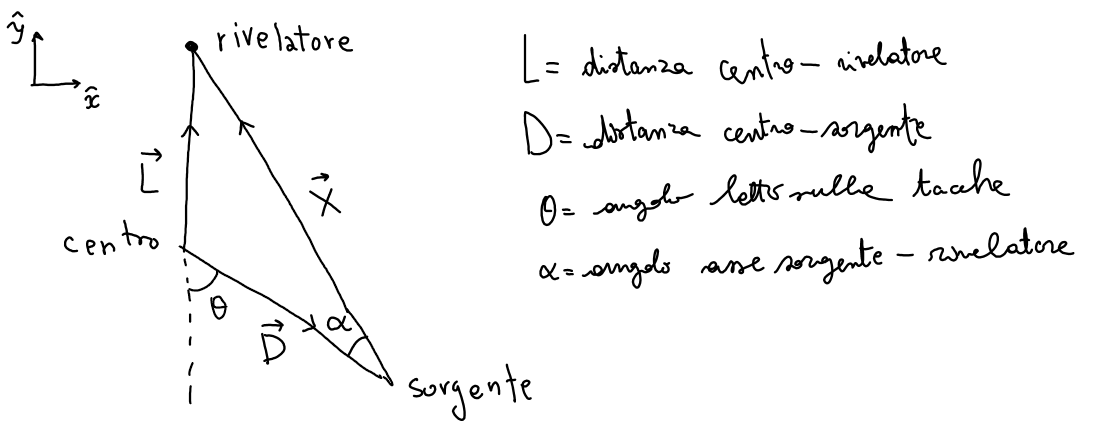
\includegraphics[width=30 em]{immagini/fma_provv}
\caption{Schema raffigurante gli angoli tra rivelatore, centro della camera a vuoto e sorgente.}
\label{fma}
\end{figure}

Applicate le dovute correzioni e usando le variabili di \autoref{fma} troviamo che l'angolo tra rivelatore e sorgente è
\begin{equation}
\cos{\alpha}= -\frac{\vec{X} \cdot \vec{D} }{ |\vec{X}| |\vec{D}| } = \frac{ L \cos{\theta} + D }{ \sqrt{ L^2+2LD\cos{\theta}+D^2  } }.
\end{equation}

Teniamo conto della variazione della distanza al variare dell'angolo moltiplicando ogni rate per $|\vec{X}|^2$.
Il risultato di questa misura è presente in \autoref{fig:forma}, i dati sono in \autoref{tab:forma}.
Nell'interpretare il grafico bisogna tener conto che per angoli abbastanza grandi
entrano in gioco il collimatore del rivelatore e la cornice della sorgente.

\begin{figure}
\centering
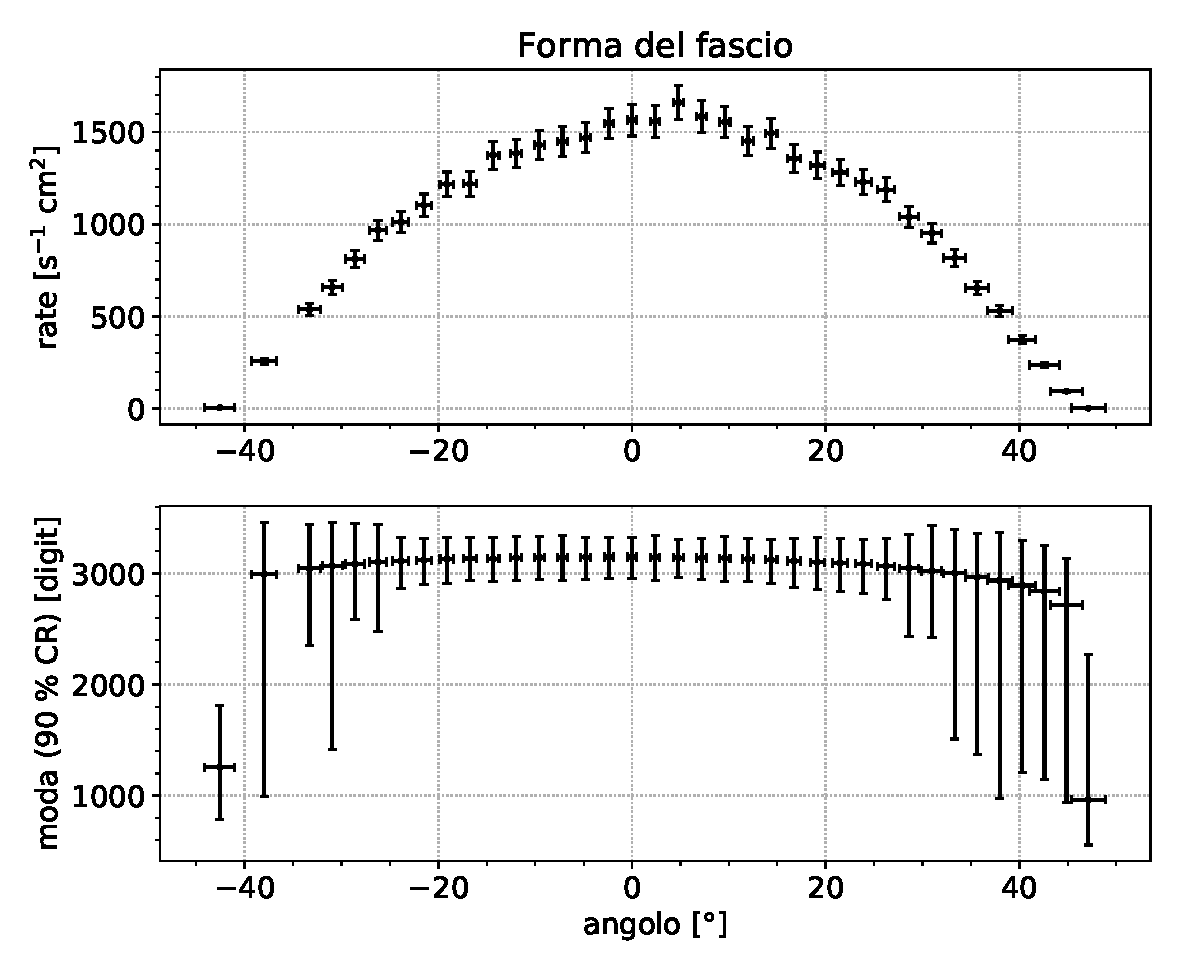
\includegraphics[width=30 em]{immagini/forma}
\caption{Sopra: rate senza bersaglio in funzione dell'angolo asse sorgente-rivelatore,
moltiplicato per la distanza al quadrato.
Le incertezze sono fortemente correlate perché includono misure di geometria dell'apparato.
Sotto: corrispondenti spettri, riportati come mode
e barre che indicano la regione che contiene il \SI{90}\% dei campioni,
ricavate con KDE.}
\label{fig:forma}
\end{figure}

\subsubsection{Collimatore da 5\! mm}

Analizziamo la forma del fascio con un collimatore da \SI{5}{mm}.
Con i dati presenti in \autoref{tab:coll5} abbiamo il grafico di \autoref{fig:coll5}.
In questo caso i conteggi sono non nulli soltanto nell'intervallo \SI{\mp10}{\degree}. La parte piatta al centro del grafico è dovuta all'effetto descritto nella sezione precedente (non corretto), ancora visibile con un'apertura di tale larghezza.

\begin{figure}[h]
\centering
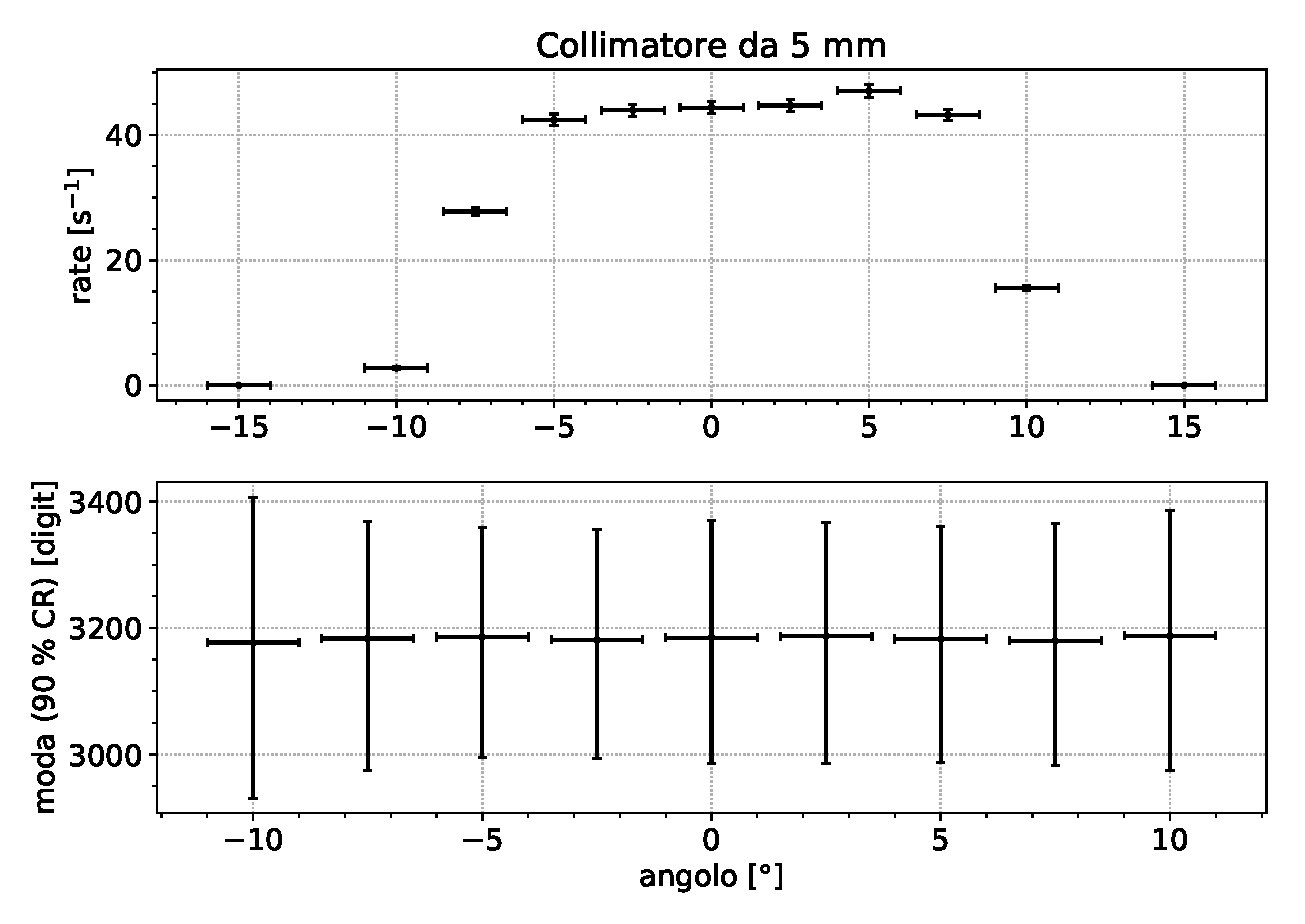
\includegraphics[width=30 em]{immagini/coll5}
\caption{Grafico del rate in funzione dell'angolo con il collimatore da 5\! mm.}
\label{fig:coll5}
\end{figure}

\subsubsection{Collimatore da 1\! mm}

Studiamo la forma del fascio con il collimatore da \SI1{mm}.
I dati sono in \autoref{tab:coll1} e \autoref{fig:coll1}.
Stavolta abbiamo conteggi solo in un intervallo di \SI{5}{\degree}.

\begin{figure}[h]
\centering
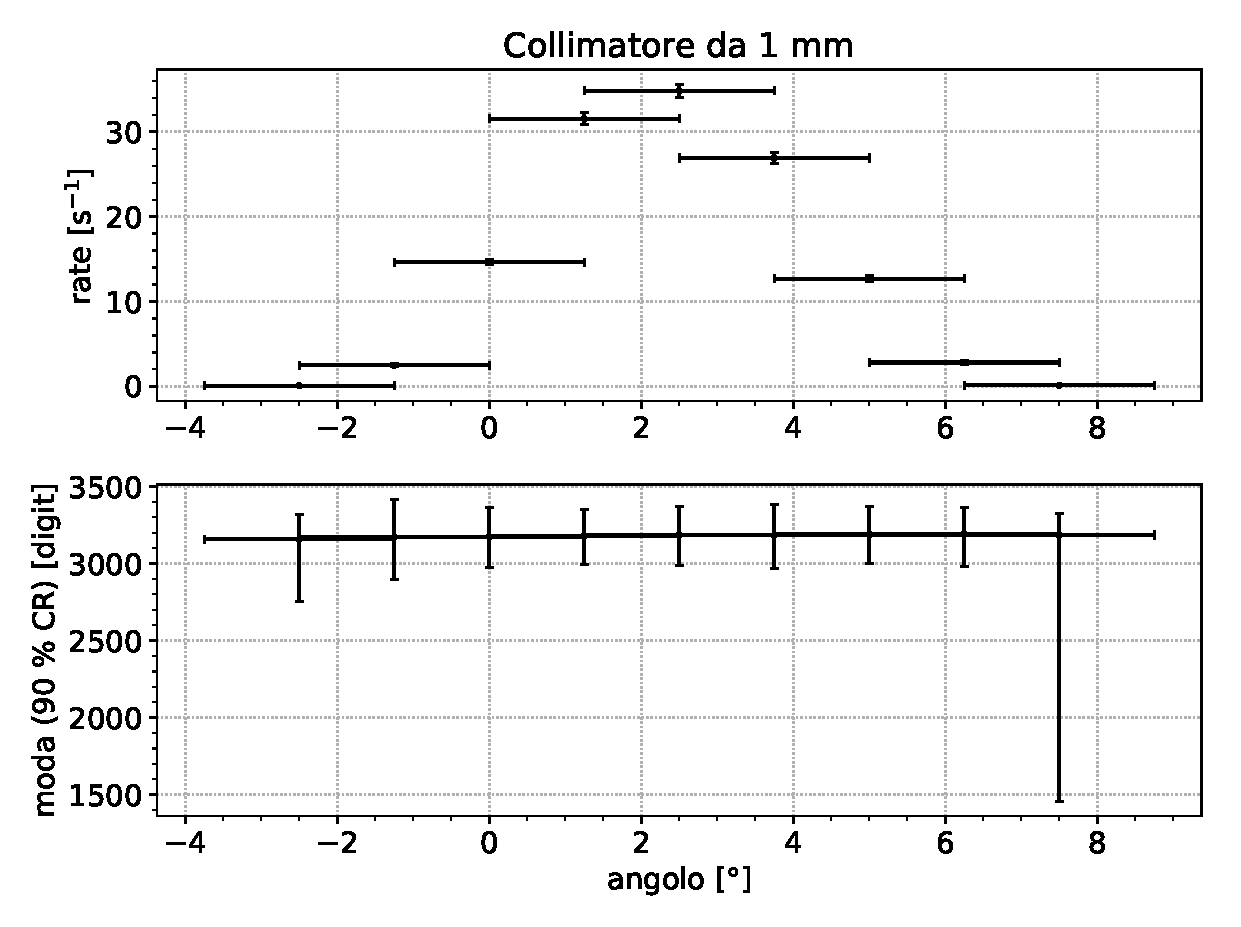
\includegraphics[width=30 em]{immagini/coll1}
\caption{Grafico del rate in funzione dell'angolo con il collimatore da 1\! mm.}
\label{fig:coll1}
\end{figure}



